\documentclass[runningheads]{llncs}

\usepackage{graphicx}
\usepackage{subcaption}
\usepackage{float}
\usepackage{biblatex}
\usepackage{censor}
\usepackage{graphicx}
\usepackage{lipsum}
\usepackage{tagging}
\usepackage[margin=4cm]{geometry}

\captionsetup{compatibility=false}
\bibliography{sota}

\usetag{draft}
\tagged{draft}{
    \usepackage{draftwatermark}
    \SetWatermarkLightness{0.9}
    \SetWatermarkScale{4}
}
\begin{document}

\tagged{redacted}{}
\untagged{redacted}{\StopCensoring}

\title{Tweet summarization methods' state of the art}

\author{Oscar Che \and
Quentin Mestre \and
Jeremy Duran \and
Jules Lamur \\
\email{\{oscar.che,quentin.mestre2,jeremy.duran,jules.lamur\}@univ-tlse3.fr}}

\authorrunning{O. Che et al.}
\institute{University of Toulouse 3 — Paul Sabatier}

\maketitle

\section{Introduction}

Social media has become a big part of our society's daily lifestyle, on average
a person has 7.6 accounts and spends 2 hours a day on social medias. In the top
5 is Twitter along with Facebook, Youtube, Instagram and Snapchat. Since its
launch in 2006, Twitter has accumulated 1.3 billion accounts with 126 million
daily active users.

The microblogging website limits its users to 280 characters per posts (or as
Twitter calls them: tweets), but that does not stop its users, as 500 million
tweets are generated each day. In fact, twitter users say and react to whatever
they like, may it be on the new Avengers trailer, videos, news or events. This
makes it a great resource for researchers attempting to build technology to
detect and summarize topics.

With the rapid growth of tweets, it is sometimes hard for users to grasp
essential information, a solution is twitter summarization. It aims to give a
concise summary from a huge amount of tweets in a given topic. Applications
could be helping users to understand topics, help agencies monitor events,
crisis progress or even disaster relief. Moreover due to the huge amount of
data and the rapidness of the information, it can also be interesting to look
into Realtime summarizations for first hand comprehension of a critical
situation.  The commerce domain is also interested in Twitter summarization,
Twitter posts being real-time messages of people raising issues, expressing
opinions, or just complaining on products, could be used by companies to get an
overall sentiment of their product.

Document summarization has been around for several years, and despite having
spawned multiple research papers, it still makes of a worthy opponent due to
the nature of tweets being opinion based and how researchers approach their
noisy-short-emoticon nature. In our state of the art we will present
summarization techniques and evaluation methods used in Twitter summarization.

\section{Topic's characteristics}

Twitter is not only a social network which provides usual ``social'' features
(such as chatting, having a profile, write freely about anything, sharing
medias, etc…), it is also the most popular microblogging platform. Nowadays, it is
really easy for one to post instantly and frequently about their own interests,
and due to this easiness: the amount of posts in microblogs became very huge
compared with that of the traditional blogs. That huge amount of data
represents a huge pool of information, however since each tweet has a short
format, the relevant information density is low and for this reason it is hard
to catch trends and public opinions on a topic. Moreover the following feature
that allows one user to follow friends, celebrities or a person that represents
huge interest from the user. Another twitter-specific feature is the
``retweet'' feature that allows the user to take someone's tweet and share it
with their followers in order to spread that tweet. All those features create
strong topic-related connections between microblogs that will increase again
the information pool. That is why summarizing is a rich and interesting field
of research in order to not be flooded by this huge amount of information.

\section{Summarization methods}

We distinguished two approaches in performing tweeter summarization: extractive
and abstractive. We will discuss about their main features, differences,
similarities and methods they used in order to produce a twitter summary.
However their relevance and quality is function of the user's appreciation and
this paper does not aim to compare them directly.

\subsection{Extractive methods}

Extractive summarization is the process of selecting sentences, words, or even
tweets (in this case) as a whole from the given data set and to put them
together. The summary can take many forms like: top tweets related on a topic,
most relevant tweet, group of tweets, group of keywords, etc… The main
feature of an extractive summary is that the content of the summary is truly
authentic.

\subsubsection{Graph based approach}

The most popular approach we encountered so far is the graph approach the goal
here is to establish a graph that represents all the sentences of selected
tweets, with all words being nodes which are related to other words.
All these nodes will be weighted by their number of occurrences in the set of
sentences. \textit{Automatic Summarization of Twitter Topics} (Sharifi et al.
2015) \cite{sharifi_automatic_nodate} describes a method based on a graph that
extracts a summary from a set of tweets/sentences.

It consists to first get all the results (tweets) of a search on a specific
topic using Twitter’s API (it returns 1500 maximum results), then it executes
the ``phase reinforcement algorithm''. This algorithm builds a graph using as
the root node the most recurrent word (or set of words). The graph is organised
from left to right, in the middle is the root node, the leafs on the left hand
side are the beginning of the sentences, and the leafs on the right hand side
are the ends of the sentences as described in the figure \ref{fig:fig1}.

\begin{figure}[H]
    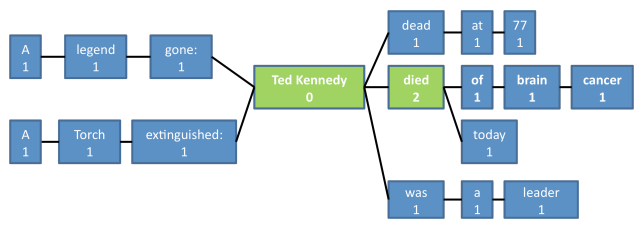
\includegraphics[width=\textwidth]{fig1.png}
    \caption{Example of a graph generated by the \textit{Automatic Summarization
    of Twitter Topics} (Sharifi et al. 2015) \cite{sharifi_automatic_nodate}
    method.}
    \label{fig:fig1}
\end{figure}

A word w of a sentence s is linked in the graph with its previous neighbor s,
and its next neighbor in s'. All nodes are weighed according to their frequency
of occurrence respective of their word ordering from the root. Now that the
graph is built, the algorithm has to find the most weighted path and then build
a new graph using the same way putting the phrase resulting to this path as the
root of the new graph. It will be repeated until the graph is not empty, the
summary is then generated.

An other way to build this graph, \textit{Entity-centric Topic-oriented Opinion
Summarization in Twitter} (Meng et al. 2012) \cite{meng_entity-centric_2012} is
by not basing the graph on words but on hashtags. This method consists in
extracting hashtags and grouping them in categories according to a category
dictionary. After classifying all the hashtags in categories we can use the
same method than before using category and not words. An example of such
categorization is shown in figure \ref{fig:fig2}.

\begin{figure}[H]
    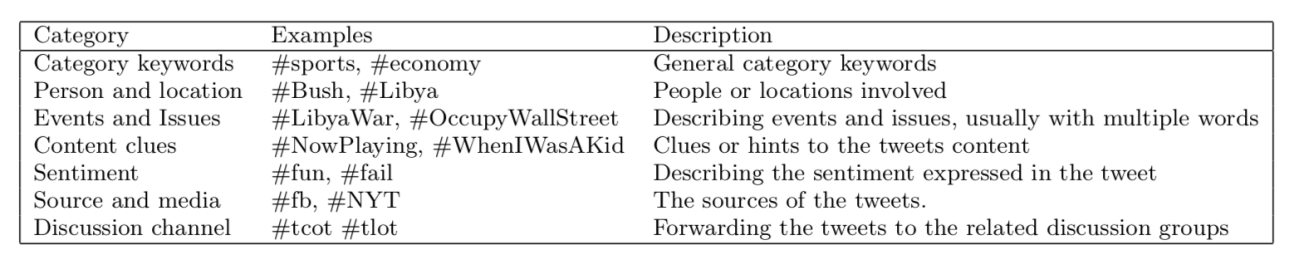
\includegraphics[width=\textwidth]{fig2.png}
    \caption{Example of a hashtags categorization
    \cite{meng_entity-centric_2012}.}
    \label{fig:fig2}
\end{figure}

\textit{Twitter Topic Summarization by Ranking Tweets using Social Influence
and Content Quality} (YaJuan et al. 2012) \cite{duan_twitter_2012} proposes
another approach of graph summarizing, their method uses the popularity of the
Twitter posters to attribute to their tweet more or less weight depending on
the popularity. They suppose that the popularity is clue of reliability.
Moreover they build a graph to refine their ranking and they used the best
tweets to generate the summary. This graph is shown in figure \ref{fig:fig3}.

\begin{figure}[H]
    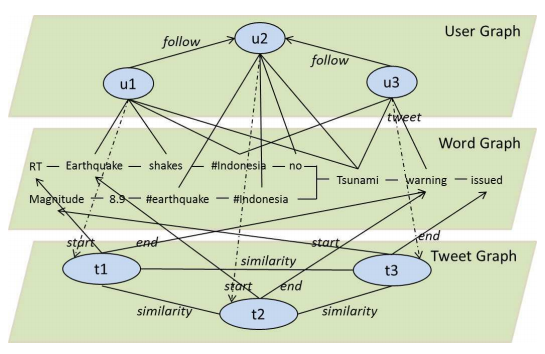
\includegraphics[width=\textwidth]{fig3.png}
    \caption{The unified mutual reinforcement graph model \cite{duan_twitter_2012}.}
    \label{fig:fig3}
\end{figure}

This graph takes into account the popularity of the user who posted this
article (the number of followers), their number of tweets concerning the topic,
and as the previous method, a graph with the words weighted by their number of
occurrences. It is a graph that gathers three sub-graphs. Afterwards, they
remove the redundancy on the selected tweets, and they apply a mathematical
formula to estimate the content quality. Once the best tweets are selected, the
paper: \textit{A Summarization Tool for Time-sensitive Social Media} (Magdy et
al. 2012)\cite{magdy_summarization_2012} proposes an interesting additional
phase of normalizing tweets to limit slang terms and special dialect terms,
this phase can enhance tweet selection.

Their approach uses English and Arabic language data sets, both languages are
rich in slang terms and different dialects, they used advanced text
normalization techniques in order to do so, but they did not named it. At the
end of this normalization process, they obtained a better summaries in various
Top tweet forms, such as Top funny tweets, top terms, top phrases, top tweets.

\subsubsection{Clustering approach}

Numerous techniques use clustering approaches in order to
produce an extractive summary. Clustering is the task of grouping a set of
objects (in this context it will be a set of tweets) that are similar. The
obtained subsets will form a cluster.

The research article \textit{A Tweet Summarization Method Based on a Keyword
Graph} (Kim et al. 2014) \cite{kim_tweet_2014} introduces a clustering approach
to produce an extractive summary. The method which is illustrated in figure
\ref{fig:fig4} consists in forming a keyword graph using the TF-IDF (Term
Frequency-Inverse Document Frequency) keywords analysis that produces a graph
of keywords. Then the K-clique Clustering method is used in order to group the
tweets. Tweets that contain all the words of that clique will have high
probability to be similar to each others and then, they are more likely to form
a cluster. This method produces as a result a cluster of tweets depending on
the keyword that the user searched for.

\begin{figure}[H]
    \centering
    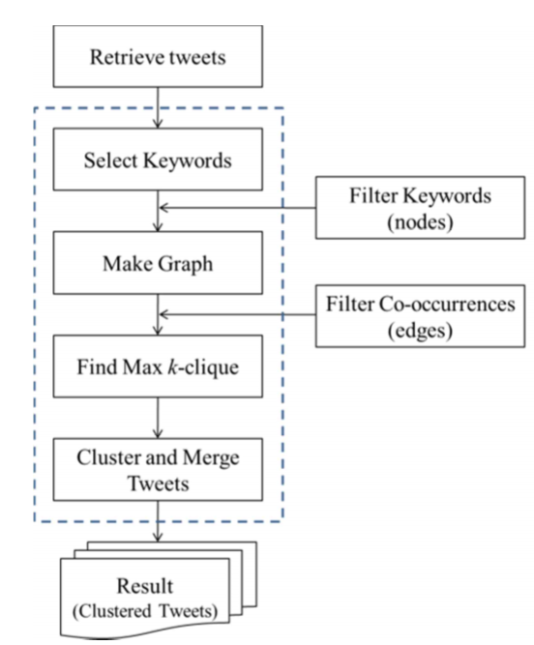
\includegraphics[width=0.5\textwidth]{fig4.png}
    \caption{Workflow of the clustering method \cite{kim_tweet_2014}.}
    \label{fig:fig4}
\end{figure}

Another approach that is worth mentionning is the method introduced in the
research \textit{A Framework for Summarizing and Analyzing Twitter Feeds} (Yang
et al. 2012) \cite{yang_framework_2012}.
The authors use a clustering approach based on a time window as illustrated in
figure \ref{fig:fig5}, their algorithm is called SPUR. Tweets are clustered into 1
hour time interval sets (they consider that tweets that were posted within 1
hour are more similar than tweets appearing 2 hours later).  They then extract
the most used sentence from that cluster and evaluate and rank each tweet by
their utility and value. At the end, they include the most relevant tweets in
their summary.

\begin{figure}[H]
    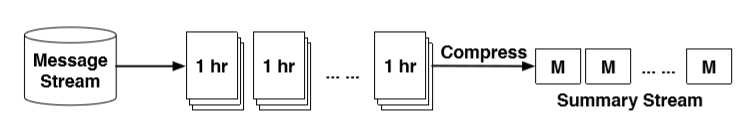
\includegraphics[width=\textwidth]{fig5.png}
    \caption{Clustering and compresson of message stream within one hour time
    window \cite{yang_framework_2012}.}
    \label{fig:fig5}
\end{figure}

\subsubsection{Statistical approach}

The article \textit{Multi-criterion Real Time Tweet Summarization Based upon
Adaptive Threshold} (Chellal et al.) \cite{chellal_multi-criterion_2016}
presents the authors's statistical method to extract tweets real time summaries
based on a user's preference.

Their method uses statistical tools which compute different statistical scores
that are then compared with adaptive thresholds. Each of the scores and
thresholds is responsible of the discrimination of the tweets that do not fit
into the summary.

The first one, called the relevance score, filters out tweets that are not
relevant for the user, based on the user's preference, known as query. The
relevance score is the number of words in common between the analyzed tweet and
the query. Secondly, the informativeness score selects tweets that bring more
information into the summary, it is computed by weighting the entropy of
Shannon of a tweet with its length. The last score is the novelty score that
detects duplicate content and aims to avoid having duplicated information. The
novelty score of an incoming tweet is a measure of its similarities to all
tweets in the current summary. The similarity is evaluated using cosine
similarity or KL-divergence.

Each score is paired with its own threshold. Except the relevance threshold
they are all adaptive, meaning that they change when the summary is updated.
The relevance threshold is a constant, two. If the tweet does not contain at
least two words of the query, it is not included in the summary.

In order to determine what are the best threshold, the authors ran tests and
experimentation on data-sets from previous TREC MB RTF contests.

The result obtained is a real time summary of a tweet stream, considering a
user interest. This summary can then be send to the user as the tweet stream is
updated. The method was evaluated and compared with other contesters methods of
the TREC MB RTF 2015 event. The authors results produced the most precise
summary of all the official runs of the event.

In another research, the authors of \textit{Light-weight, Conservative yet
Effective: Scalable Real-time Tweet Summarization} (Suwaileh et al. in 2016)
\cite{suwaileh_light-weight_nodate} used another similar filtering pipeline
with again and relevance, novelty filters. The results were well graded during
the TREC MB RTF 2016 contest.

\subsection{Abstractive methods}

Abstractive summaries are generated sentences based on semantic understanding.
Such summaries contain sentences that may not appear in the input data, the
goal here is to generate human-understandable sentences with high information
density so the user has a global idea of what is happening while decreasing his
search efforts. We can see extractive methods as a process of selecting while
abstractive methods is a rather reformulating approach. We must notify that
those methods are fewer than the extractives one.

\subsubsection{Graph based approach}

The summarizations methods that will be presented here will not much differ
from the one presented in the Extractive section, but it is interesting to see
how their summaries differ. We will have a look on \textit{Efficient Online
Summarization of Microblogging Streams} (Olariu 2014)
\cite{olariu_efficient_2014}, and its Twitter Online Word Graph Summarizer
(TOWGS), this approach is interesting because it does not save any of the
tweets, it also skips any clustering steps, they instead build word graphs from
tri-grams (n-grams of words), each tri-grams will represent a node and their
corresponding edges will be weighted based on the frequencies of that trigram
related to the tweets. But the more important part is that this method is
Online (real time), in the previous techniques we presented the word graphs
were discarded after generating the summary, that is not the case here: for the
online summary, the graph is constantly updated with tweets and their initial
word graph ``forget'' the old data via a time decaying window. Then in order to
generate an abstractive summary this technique looks for the highest scoring
path by using a greedy search strategy in the graph, this path connects the
special words which marks the beginning and the end of the sentence and
proposes an updated summary sentence as a result. TOWGS method is a real
contender for the most advanced abstractive real time method on tweets
summarization. As we said earlier, abstractive approaches are generating
sentences, those sentences can sometimes be difficult for the users to read.
The following method insists on making grammatically correct sentences
\textit{Better Twitter Summaries ?} (Judd et al. 2013) \cite{judd_better_2013}
proposed in their paper a revisited PR algorithm, their main idea is to build a
Governor/Dependent dependence between words in a sentence in order to produce
better summaries. Sometimes the classic PR algorithm can produce the following
abstract summary: ``today is day for vote Obama this election day'' (taken
from the article) which is not correct. In order to fix that sentence they will
first classify words and then apply their revisited PR algorithm (see figure
\ref{fig:fig6} and figure \ref{fig:fig7}). At the end of this process, a supposed
grammatically correct sentence is formed.

\begin{figure}
    \centering
    \begin{subfigure}[b]{0.4\textwidth}
        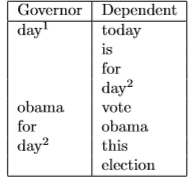
\includegraphics[width=\textwidth]{fig6.png}
        \caption{Governor dependent word labeling.}
        \label{fig:fig6}
    \end{subfigure}
    ~
    \begin{subfigure}[b]{0.4\textwidth}
        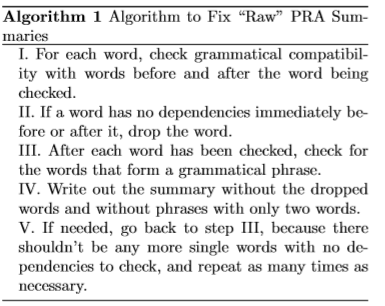
\includegraphics[width=\textwidth]{fig7.png}
        \caption{Revisited PR algorithm.}
        \label{fig:fig7}
    \end{subfigure}
    \caption{\cite{judd_better_2013}}
\end{figure}

\subsubsection{Others}

There are alternative ways to create abstract summaries different from graph or
clustered approaches, a paper from Nilambari Maruti Dhanve from the Solapur
University in India, uses Speech Acts in their article \textit{Twitter Trending
Topic Summarization Using Speech Act} (Dhanve et al.
2007) \cite{dhanve_twitter_2007} for their abstractive summarization.
A Speech Act is something expressed by an individual that not only presents
information, but performs an action as well. For example ``Hi, Eric. How are
things going?'' is performing the action of Greeting, and ``Could you pass me
the ranch, please ?'' corresponds to a request. With a data set, the research
team extracts phrases (n-grams) and assigns them to the corresponding speech
act. They then implement a ranking to the words and select the most salient
ones for the summary see figure \ref{fig:fig8}. The selected are inserted into
proper slots of speech act-guided templates to generate abstractive summaries.

\begin{figure}[H]
    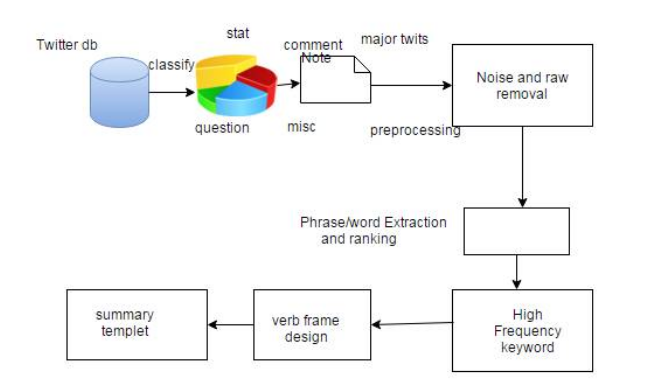
\includegraphics[width=\textwidth]{fig8.png}
    \caption{Workflow used in speech act \cite{dhanve_twitter_2007}.}
    \label{fig:fig8}
\end{figure}

\section{Evaluation methods}

Evaluation of twitter summaries is not an easy task for several reasons, as we
saw previously there are different kinds of summaries and also there is not
only one correct summary for a given topic. Knowning that, it becomes
difficult to have a real standard evaluation method for every twitter
summarizations, still, there are evaluation methods that can assess one's
summary content quality by grammar, readability, cohesiveness of the content.
It is actually possible to have some reference metrics or any kind of approach
for evaluation. In this section we will discuss about the main evaluation
methods we encountered so far.

\subsection{Evaluation metrics}

We present here the most important metrics we encountered in the literature in
order to assess and give objective evaluation on twitter summaries results.

\subsubsection{ROUGE}

The most famous and used evaluation method for summarizations is certainly ROUGE
metrics. ROUGE stands for Recall-Oriented Understudy for Gisting Evaluation, it
is in fact a set of metrics. Most of the summarizations methods we saw earlier
are using ROUGE metrics in order to assess their generated summaries.
The evaluation method compares a generated summary against a set of references
summaries (mainly human produced) then it computes metrics on this comparaison
such as Recall metric (number of overlapping words divided by total word in
reference summary) and precision metric (number of overlapping words divided by
total relevant words). In order to have a better evaluation and to fit more into
different summaries, alternative versions of ROUGE exist, such as ROUGE-N
(where the evaluation is emphasized on n-gram measure), ROUGE-L (measures
longest matching sequence of words), ROUGE-S (count number of word in the right
order). From our reading experience, we noticed that ROUGE-1 was the most used
one, the reason is that tweet summaries are short and very concise, so ROUGE-1
is sufficient enough to produce a good assessment on twitter summaries. It
happens that the researchers use multiple evaluation method to have a better
overview of their approach's performances as it was done in \textit{Twitter
Summarization Based on Social Network and Sparse Reconstruction} (He et al.
2018) \cite{he_twitter_nodate}.

\subsubsection{F-Measure}

F-measure (F1-score or F-score) is a measure of a test's accuracy and is
defined as the weighted harmonic mean of the precision and recall of the test,
the F measure is often used in information retrieval for measuring search,
document classification, and query classification, performance and clustering
approaches as we saw in numerous papers.The F-value varies between 0 and
1(which is the best score).\textit{Automatic Summarization of Tweets in
Providing Indonesian Trending Topic} (Winatmoko et al. in 2013)
\cite{winatmoko_automatic_2013} uses a F-measure to compare their solution with
Sumbasic (Vanderwende et al. 2007) \cite{vanderwende_beyond_2007} and Hybrid
TF-IDF (Inouye and Kalita 2011) \cite{inouye_comparing_2011} summarization
solution. Or else \textit{A Tweet Summarization Method Based on a Keyword
Graph} (Kim et al. in 2014) \cite{kim_tweet_2014} uses this evaluation method
to compare their results with the STC algorithm.

\subsubsection{Gain metrics}

Most of statistics based approaches (Suwaileh et al. in 2016)
\cite{suwaileh_light-weight_nodate} and (Chellal et al. in 2016)
\cite{chellal_multi-criterion_2016} of tweets summarization use a special
evaluation that refers to multiple evaluation measures to wit expected gain
(EG), normalized cumulative gain (nCG), gain minus pain (GMP) and/or expected
latency-discounted gain (ELG), it is the average of all these results that is
used for evaluation.

\subsection{Evaluation campaigns}

Entities such as universities, private companies, and/or state decide to
co-operate and launch big conferences. Those conferences are in fact big
workshops that aim to encourage research in a specific domain. The main goal
for those conferences is to improve relationships between industries and the
research domain, accelerate knowledge transfers between researchers and
industry for commercial purposes and also development of new evaluations
techniques that will fit better new technologies.

\subsubsection{TREC}

The main evaluation campaign that concern our topic here is TREC, it stands for
Text REtrieval Conference and its first goal is to support research within the
information retrieval community, by providing the infrastructure necessary for
large-scale evaluation of text retrieval methodologies.

TREC takes place once a year and is sponsored by the United States of America
and NIST(National Institute of Standards and Technology), NIST will provide to
each participant a test set and some questions, then every participant can try
whatever approach they estimate worthy to try in order to answer the questions.
Once the results processed, NIST retrieves them, judges and evaluates the
results in function of the correctness.

With the constant growth of interest in TREC and the number of participants
growing each year, TREC's evaluation campaigns became a reference in text
retrieval research and the TREC's test collections and  evaluation software
were made available publicly so more organizations can assess their methods. We
must notify that the only paper we read concerning twitter summarization which
participated in a TREC iteration was the \textit{Multi-criterion Real Time
Tweet Summarization Based Upon Adaptive Threshold} (Chellal et al. in 2016)
\cite{chellal_multi-criterion_2016}.

\subsubsection{Human evaluation}

A different approach to evaluation is to use humans to score a given summary.
There exists two types of evaluation with human assistance, human readers, who
compare the summary with a given summary and human judges, that pick sentences
that best summarize the topic.  Human readers are used to measure a machine
generated summary to a reference summary with a point system, the reference
summary being man made. Human judges pick out sentences that give the best
information for a given topic. The effectiveness of these methods depend on the
humans, it generally occurs that different humans have different understandings
of a topic. It is also frequent that the human may have a different
understanding of the subject later on. Hongyan Jing et al. in 1998
\cite{jing_summarization_nodate} shows throughout their paper that multitude
parameters influence the human evaluation method and that one is not more
applicable then the other. For example, the reliability of an evaluation
decreases with the length of a summary. However setting the best parameters
strengthens their outcome and users should choose according to their needs.

\section{Conclusion}

Twitter rapidly became the most important source of information all over the
world, it even overtook classic medias such as newspaper, magazines, TV news or
general blogs. However grasping important information is sometimes a difficult
task. This being said, Twitter summarization represents an important research
field and in our paper we presented an overview of what has been done today in
order to generate Twitter summaries following two axes: extractive and
abstractive summarization. We also presented the most prominent evaluation
methods to assess generated summaries, while evaluation of Twitter summaries is
not standardized yet it seems to converge towards using the same metrics: the
ROUGE method. With Twitter's number of users growing everyday, and to avoid fake
news spreading phenomenon, the next challenge for Twitter summarization could
be to check the integrity and reliability of the information in order to
produce more trustable summaries.

\printbibliography

\end{document}
